%Đây là template dùng cho đề cương đề tài tốt nghiệp
%Khoa Công nghệ Thông tin
%Trường Đại học Khoa học Tự nhiên, ĐHQG-HCM

%Liên hệ về mẫu LaTEX này: Thầy Bùi Huy Thông (bhthong@fit.hcmus.edu.vn)

\documentclass[14pt]{article}  % Sửa: đối số tùy chọn phải đứng trước tên lớp
\usepackage[utf8]{vietnam}
\usepackage{enumerate}
\usepackage{enumitem}
\usepackage{multicol}
\usepackage{listings}
\usepackage[left=2cm,right=2cm,top=2.5cm,bottom=2.5cm]{geometry}
\usepackage{verbatim}
\usepackage{graphicx}
\usepackage{url}
\usepackage{fancyhdr}
\usepackage{fancybox,framed}
\linespread{1.3}
\usepackage{lastpage}
\usepackage{floatrow}  % Sửa: bỏ khai báo trùng lặp
\usepackage{float}
\floatsetup[table]{capposition=top}
\usepackage{booktabs}
\pagenumbering{arabic}
%\pagestyle{fancy}
\newfloatcommand{capbtabbox}{table}[][\FBwidth]

\usepackage{blindtext}
\usepackage{titlesec}
\usepackage{amsmath}
\usepackage{amssymb}
\usepackage{url}
\usepackage[colorlinks=true, linkcolor=blue, citecolor=blue, urlcolor=blue]{hyperref}

\titleformat*{\section}{\LARGE\bfseries}
\titleformat*{\subsection}{\Large\bfseries}
\titleformat*{\subsubsection}{\large\bfseries}


\begin{document}
    \begin{figure}[h]
        \begin{floatrow}
        \ffigbox{
\includegraphics[scale = .4]{logo.png}}
        {%

        }
        \capbtabbox{
            \begin{tabular}{l}
            \multicolumn{1}{c}{\textbf{\begin{tabular}[c]{@{}c@{}}TRƯỜNG ĐẠI HỌC KHOA HỌC TỰ NHIÊN\\KHOA CÔNG NGHỆ THÔNG TIN\end{tabular}}} \\ \\ \\
            \end{tabular}
        }
        {%

        }
        \end{floatrow}
    \end{figure}

    \begin{center}
        %Xác định loại đề tài tốt nghiệp tương ứng: Khóa luận, Thực tập, Đồ án
        \textbf{\Large ĐỀ CƯƠNG KHOÁ LUẬN TỐT NGHIỆP} \\
    \end{center}

    \begin{center}
    %Tên đề tài phải VIẾT HOA
        \textbf{\huge XÂY DỰNG MẠNG NƠ-RON LAI LƯỢNG TỬ -- CỔ ĐIỂN DỰA TRÊN KIẾN TRÚC U-NET CHO BÀI TOÁN PHÂN ĐOẠN ẢNH Y SINH}
        \\

    %Tên đề tài bằng tiếng Anh (nếu có)
    \vspace{.5cm}
        \textit{\textbf{\Large DEVELOPING A HYBRID QUANTUM-CLASSICAL U-NET ARCHITECTURE FOR BIOMEDICAL IMAGE SEGMENTATION}}
    \end{center}

    \vspace{.5cm}

    \Large
    \section{THÔNG TIN CHUNG}
    \begin{itemize}[label = {}]

        \item \textbf{Người hướng dẫn:}
        %Thể hiện dạng: <Chức danh> <Họ và tên> (<Đơn vị công tác>)
        \begin{itemize}
            \item ThS. Phạm Trọng Nghĩa (Khoa Công nghệ Thông tin)
            \item ThS. Lê Nhựt Nam (Khoa Công nghệ Thông tin)
        \end{itemize}{}


        \item \textbf{Nhóm sinh viên thực hiện:}

        %Thể hiện dạng: <Họ và tên sinh viên> (MSSV: )
        \begin{enumerate}

            \item Nguyễn Sinh Trực (MSSV: 22120395)
            \item Phạm Tuấn Vương (MSSV: 22120446)
        \end{enumerate}

       %Chọn loại thích hợp
        \item \textbf{Loại đề tài:} Nghiên cứu

        \item \textbf{Thời gian thực hiện:} Từ \textit{01/2026} đến \textit{07/2026}


    \end{itemize}

    \pagebreak

    \section{NỘI DUNG THỰC HIỆN}
    {

    %Mỗi mục dưới đây phải viết ít nhất là 5 câu mô tả/giới thiệu.

    \subsection{Giới thiệu về đề tài}

    Trong lĩnh vực y tế, việc phân đoạn chính xác các vùng tổn thương hoặc cấu trúc giải phẫu từ ảnh y sinh đóng vai trò then chốt trong chẩn đoán lâm sàng, lập kế hoạch điều trị và theo dõi tiến triển bệnh. Khác với bài toán phân loại ảnh chỉ gán một nhãn duy nhất cho toàn bộ ảnh, bài toán phân đoạn ảnh y sinh (biomedical image segmentation) yêu cầu xác định nhãn cho từng điểm ảnh riêng lẻ, từ đó xác định chính xác vị trí và hình dạng của vùng tổn thương ở mức độ chi tiết hơn nhiều. Độ chính xác của quá trình khoanh vùng ranh giới tổn thương có ảnh hưởng trực tiếp đến hiệu quả điều trị, đặc biệt trong các bệnh lý phức tạp như ung thư hắc tố (melanoma) hay ung thư đại trực tràng. Tuy nhiên, việc phân đoạn thủ công đòi hỏi chuyên môn cao, tốn nhiều thời gian và dễ thiếu nhất quán do phụ thuộc chủ quan người thực hiện, đặt ra nhu cầu về các phương pháp phân đoạn tự động, chính xác.

    Kiến trúc U-Net \cite{ronneberger2015unet} với cấu trúc đối xứng Encoder--Bottleneck--Decoder và các skip connections đã trở thành nền tảng chuẩn mực cho phân đoạn ảnh y sinh, đạt hiệu quả cao ngay cả khi dữ liệu hạn chế nhờ bảo tồn chi tiết không gian. Tuy nhiên, các lớp tích chập cổ điển còn hạn chế trong việc biểu diễn các tương quan phi tuyến phức tạp, đặc biệt tại vùng Bottleneck ở độ phân giải thấp nhất -- đặt ra nhu cầu bổ sung cơ chế trích xuất đặc trưng mạnh hơn tại vùng này.

    Sự phát triển của điện toán lượng tử trong những năm gần đây đã mở ra những hướng tiếp cận mới cho học máy thông qua các phương pháp học máy lượng tử (Quantum Machine Learning -- QML) \cite{biamonte2017qml}. Một trong những hướng hứa hẹn nhất là xây dựng các mô hình lai lượng tử -- cổ điển (Hybrid Quantum-Classical models), trong đó các mạch lượng tử tham số hóa (Parametrized Quantum Circuit -- PQC) được tích hợp như những thành phần bổ sung vào kiến trúc học sâu cổ điển, nhằm tận dụng các tính chất đặc trưng của cơ học lượng tử như chồng chất (superposition) và vướng víu lượng tử (entanglement) để mở rộng không gian biểu diễn đặc trưng \cite{du2025qmltutorial}. Đặc biệt, module QuFeX (Quantum Feature Extraction module) đã được đề xuất như một khối tính toán lai có thể tích hợp linh hoạt vào các kiến trúc mạng nơ-ron học sâu hiện có, cho phép biểu diễn đặc trưng trong không gian Hilbert lượng tử với số chiều tăng trưởng theo hàm mũ so với số qubit sử dụng \cite{qufex2025}. Các nghiên cứu về mạng nơ-ron lai như Quanvolutional Neural Networks \cite{henderson2020quanvolution} và các kiến trúc hybrid quantum-classical trong phân loại ảnh y khoa \cite{shahjalal2025hqcnn} đã bước đầu chứng minh tiềm năng của việc tích hợp thành phần lượng tử vào học sâu cổ điển. Tuy nhiên, hướng ứng dụng của các mô hình lai này cho bài toán phân đoạn ảnh y sinh -- đặc biệt là tích hợp module QuFeX vào kiến trúc encoder-decoder dạng U-Net -- vẫn còn ít được nghiên cứu và cần được khảo sát thêm.

    Xuất phát từ những vấn đề trên, đề tài xây dựng một kiến trúc lai lượng tử -- cổ điển dựa trên U-Net cho phân đoạn ảnh y sinh. Khởi đi từ ý tưởng của module QuFeX \cite{qufex2025}, đề tài đề xuất một khối lượng tử mạnh hơn tại Bottleneck theo cơ chế hỗn hợp nhánh xử lý lượng tử đa tỷ lệ (Quantum Mixture of Experts), tiếp nối bởi một khối chuỗi lấy cảm hứng từ Mamba \cite{gu2023mamba} để tổng hợp phụ thuộc không gian tầm xa với chi phí tuyến tính, đồng thời tăng cường bộ khung cổ điển bằng một khối tích chập đa tỷ lệ giãn nở (RDMS) ở các tầng Encoder--Decoder. Kiến trúc được đánh giá bằng các chỉ số IoU và Dice, so sánh với các mô hình cổ điển (U-Net, UNet++, Attention U-Net, V-Net, R2U-Net) và mô hình lai dựa trên QuFeX trên hai tập PH2 và GlaS 2015, trong điều kiện giả lập của kỷ nguyên NISQ \cite{vu2025quantum}.

    \subsection{Mục tiêu đề tài}

    %Phần này mô tả về động lực để giải quyết vấn đề.
    Các kiến trúc học sâu như U-Net, Attention U-Net và UNet++ đã đạt kết quả ấn tượng trong phân đoạn ảnh y sinh, song vẫn còn giới hạn về khả năng biểu diễn đặc trưng toàn cục tại vùng Bottleneck, nhất là khi dữ liệu hạn chế hoặc đối tượng có ranh giới mờ. Học máy lượng tử -- điển hình là module QuFeX \cite{qufex2025} -- mở ra hướng tăng cường trích xuất đặc trưng trong không gian Hilbert cho chính vùng này.

    Xuất phát từ những vấn đề trên, đề tài này hướng đến việc nghiên cứu và xây dựng một kiến trúc Hybrid Quantum-Classical U-Net, trong đó vùng Bottleneck được tăng cường bằng một khối hỗn hợp nhánh xử lý lượng tử đa tỷ lệ kết hợp với một khối mô hình hóa chuỗi lấy cảm hứng từ Mamba, cùng một khối tích chập đa tỷ lệ giãn nở (RDMS) tăng cường bộ khung cổ điển, nhằm nâng cao khả năng biểu diễn và tổng hợp đặc trưng cho bài toán phân đoạn ảnh y sinh. Trọng tâm chính của đề tài là thiết kế và đánh giá kiến trúc mạng lai này thông qua thực nghiệm trên hai tập dữ liệu y sinh PH2 và GlaS 2015.

    Cụ thể, các mục tiêu chính của đề tài bao gồm:
    \begin{itemize}
        \item Nghiên cứu kiến trúc U-Net và các biến thể, cùng các phương pháp tích hợp thành phần lượng tử vào học sâu (mã hóa dữ liệu, PQC, đo lường; điển hình QuFeX \cite{qufex2025}).
        \item Đề xuất và hiện thực khối lượng tử tại Bottleneck theo cơ chế hỗn hợp nhánh xử lý lượng tử đa tỷ lệ, kết hợp khối chuỗi lấy cảm hứng từ Mamba \cite{gu2023mamba} tổng hợp phụ thuộc tầm xa với chi phí tuyến tính, và khối tích chập đa tỷ lệ giãn nở (RDMS) ở bộ khung cổ điển.
        \item Đánh giá, so sánh với các mô hình cổ điển (U-Net, UNet++, Attention U-Net, V-Net, R2U-Net) và mô hình lai QuFeX qua IoU/Dice, và phân tích ảnh hưởng của các yếu tố thiết kế (số qubit, số nhánh xử lý) \cite{du2025qmltutorial}.
    \end{itemize}

    Kết quả được kỳ vọng cung cấp bằng chứng thực nghiệm về tính khả thi và giá trị của việc kết hợp hỗn hợp nhánh xử lý lượng tử với mô hình hóa chuỗi hiệu quả tại vùng Bottleneck của U-Net cho phân đoạn ảnh y sinh.

    \subsection{Phạm vi của đề tài}

    \subsubsection{Nội dung nghiên cứu chính}

    \textbf{Kiến trúc Hybrid Quantum-Classical U-Net:} Đề xuất và hiện thực khối lượng tử tại Bottleneck theo cơ chế hỗn hợp nhánh xử lý lượng tử đa tỷ lệ kết hợp khối chuỗi lấy cảm hứng từ Mamba, cùng một khối tích chập đa tỷ lệ giãn nở (RDMS) tăng cường bộ khung cổ điển, đánh giá trên môi trường giả lập lượng tử phù hợp điều kiện NISQ.

    \textbf{Thành phần lượng tử:} Nghiên cứu các cơ chế trích xuất đặc trưng lượng tử (mã hóa dữ liệu, PQC, đo lường; điển hình là QuFeX \cite{qufex2025}), từ đó thiết kế khối hỗn hợp nhánh xử lý lượng tử đa tỷ lệ trong đó mỗi nhánh xử lý một mảnh ảnh không gian với kích thước và số qubit khác nhau, được điều phối bởi mạng định tuyến cổ điển.

    \textbf{Hệ thống các chỉ số đánh giá:} Xây dựng bộ tiêu chí đánh giá bao gồm các chỉ số chuyên dụng cho bài toán phân đoạn ảnh như Intersection over Union (IoU), Dice Coefficient (DSC), Precision, Recall (Sensitivity) và Specificity tính trên từng điểm ảnh. Bên cạnh đó, tiến hành so sánh kiến trúc lai đề xuất với các mô hình cổ điển (U-Net, UNet++, Attention U-Net, V-Net, R2U-Net) và mô hình lai dựa trên QuFeX nhằm đánh giá mức độ cải thiện của phương pháp.

    \subsubsection{Đối tượng nghiên cứu và thực thể liên quan}

    \textbf{Đối tượng nghiên cứu:} Kiến trúc mạng nơ-ron lai lượng tử -- cổ điển dựa trên U-Net với khối hỗn hợp nhánh xử lý lượng tử, khối LSS (lấy cảm hứng từ Mamba) tại Bottleneck và khối RDMS (tích chập đa tỷ lệ giãn nở) ở bộ khung cổ điển, được ứng dụng cho bài toán phân đoạn ảnh y sinh với nhãn ở mức pixel.

    \textbf{Thực thể liên quan:}

    \begin{itemize}
        \item Mô hình học sâu cổ điển: U-Net \cite{ronneberger2015unet}, UNet++ \cite{zhou2018unetplusplus}, Attention U-Net \cite{oktay2018attention}, V-Net \cite{milletari2016vnet} và R2U-Net \cite{alom2018r2unet} làm mô hình đối chứng.
        \item Thành phần lượng tử: module trích xuất đặc trưng lượng tử QuFeX \cite{qufex2025} và cơ chế hỗn hợp nhánh xử lý lượng tử đề xuất.
        \item Khối mô hình hóa chuỗi: khối lấy cảm hứng từ Mamba \cite{gu2023mamba} tổng hợp phụ thuộc không gian tầm xa.
        \item Khối tích chập đa tỷ lệ cổ điển: khối RDMS (Residual Dilated Multi-Scale) tăng cường trường nhìn ở bộ khung Encoder--Decoder.
        \item Mô hình lai: kiến trúc lai đề xuất và mô hình lai dựa trên QuFeX dùng để so sánh.
    \end{itemize}

    \textbf{Tập dữ liệu:} Đề tài sử dụng hai tập dữ liệu y sinh với hai phương thức hình ảnh khác nhau nhằm đánh giá khả năng tổng quát hóa, bao gồm tập \textit{PH2} (ảnh dermoscopy) và tập \textit{GlaS 2015} (ảnh mô học đại trực tràng nhuộm H\&E). Cả hai tập đều cung cấp các cặp ảnh gốc kèm mặt nạ phân đoạn nhị phân (\textit{ground-truth mask}) được chú thích ở mức pixel, trong đó vùng đối tượng được đánh dấu bằng giá trị 1 và phần nền bằng giá trị 0.

    \textbf{Tập PH2} \cite{mendonca2013ph2}: gồm 200 ảnh dermoscopy màu (Bệnh viện Pedro Hispano, Bồ Đào Nha) kèm mặt nạ tổn thương da, trải trên ba nhóm chẩn đoán (nốt ruồi thường, không điển hình và melanoma). Quy mô nhỏ khiến PH2 phù hợp để đánh giá mô hình trong điều kiện dữ liệu hạn chế -- nơi kiến trúc lai lượng tử được kỳ vọng có lợi thế.

    \textbf{Tập GlaS 2015} \cite{sirinukunwattana2017glas}: bộ ảnh Warwick-QU của thách thức phân đoạn tuyến tại MICCAI 2015, gồm 165 ảnh mô học nhuộm H\&E của mô đại trực tràng kèm mặt nạ vùng tuyến ở mức pixel. Khác với PH2, GlaS chứa nhiều tuyến có hình thái đa dạng, ranh giới phức tạp và nền mô đệm nhiễu, tạo một điều kiện đánh giá tương phản mạnh với PH2.

    Trong quá trình tiền xử lý, tất cả ảnh từ cả hai tập dữ liệu được chuẩn hóa về kích thước đồng nhất $192 \times 256$ pixel và đưa giá trị điểm ảnh về đoạn $[0,1]$. Mặt nạ phân đoạn cũng trải qua đúng quy trình biến đổi hình học tương ứng với ảnh để đảm bảo tính nhất quán trong từng cặp dữ liệu.

    \textbf{Công cụ và môi trường thực nghiệm:} Python, TensorFlow/Keras và thư viện giả lập lượng tử PennyLane (thiết bị \texttt{default.qubit}) để hiện thực các thành phần lượng tử và tích hợp chúng vào mạng nơ-ron học sâu thông qua cơ chế tự động vi phân, hỗ trợ lan truyền ngược gradient xuyên suốt phần lượng tử và cổ điển.

    \subsubsection{Các giới hạn và ràng buộc của đề tài}

    Đề tài giới hạn ở phân đoạn ảnh y sinh 2D trên hai phương thức (dermoscopy và mô học), chưa mở rộng sang ảnh khối 3D. Do điều kiện NISQ, số qubit và độ sâu mạch lượng tử phải được giới hạn ở mức phù hợp; toàn bộ thành phần lượng tử được triển khai và đánh giá trên môi trường \emph{giả lập} (\texttt{default.qubit}), chưa chạy trên phần cứng lượng tử thực.

    \subsection{Cách tiếp cận dự kiến}

\subsubsection{Cơ sở phương pháp và các nghiên cứu liên quan}

Kiến trúc U-Net \cite{ronneberger2015unet} với hai nhánh Encoder--Decoder đối xứng và các skip connections là nền tảng của phần lớn hệ thống phân đoạn ảnh y sinh; vùng Bottleneck ở độ phân giải thấp nhất là nơi tập trung ngữ nghĩa toàn cục nhất, và do đó là vị trí chiến lược để bổ sung các cơ chế trích xuất đặc trưng tiên tiến hơn.

Trong học máy lượng tử, nhiều nghiên cứu đã chỉ ra tiềm năng của các mạch lượng tử tham số hóa (PQC) trong việc biểu diễn các lớp hàm phức tạp \cite{biamonte2017qml}; các mô hình lai như Quanvolution \cite{henderson2020quanvolution}, QCQ-CNN \cite{long2025qcq} và HQCNN cho phân loại ảnh y khoa \cite{shahjalal2025hqcnn} đã bước đầu chứng minh lợi ích của việc tích hợp thành phần lượng tử vào học sâu, đặc biệt với dữ liệu hạn chế. Gần đây, module QuFeX \cite{qufex2025} đề xuất một khối trích xuất đặc trưng lượng tử dạng \textit{plug-and-play} theo ba giai đoạn (mã hóa dữ liệu $\to$ PQC $\to$ đo lường), có thể nhúng vào vùng Bottleneck của U-Net -- được đề tài lấy làm điểm khởi đầu tham chiếu.

\subsubsection{Phương pháp tiếp cận đề xuất}

Dựa trên các hướng trên, đề tài xây dựng một kiến trúc Hybrid Quantum-Classical U-Net giữ nguyên Encoder--Decoder cổ điển, thay thế khối xử lý tại Bottleneck bằng: (i) một khối hỗn hợp nhánh xử lý lượng tử đa tỷ lệ -- nhiều mạch PQC xử lý các mảnh không gian ở nhiều tỷ lệ, điều phối bởi một mạng định tuyến Softmax và kết nối residual -- tiếp nối bởi (ii) một khối chuỗi lấy cảm hứng từ Mamba tổng hợp phụ thuộc không gian tầm xa với chi phí tuyến tính \cite{gu2023mamba}, đồng thời tăng cường bộ khung Encoder--Decoder bằng (iii) một khối tích chập đa tỷ lệ giãn nở có phần dư (RDMS) để mở rộng trường nhìn mà không tăng đáng kể số tham số. Nguyên tắc chỉ can thiệp tại Bottleneck và bộ khung giúp hạn chế chi phí tính toán tăng thêm mà vẫn kế thừa năng lực phân đoạn đã kiểm chứng của U-Net. Hình~\ref{fig:overview_proposal} minh họa tổng quan kiến trúc lai đề xuất.

\begin{figure}[H]
    \centering
    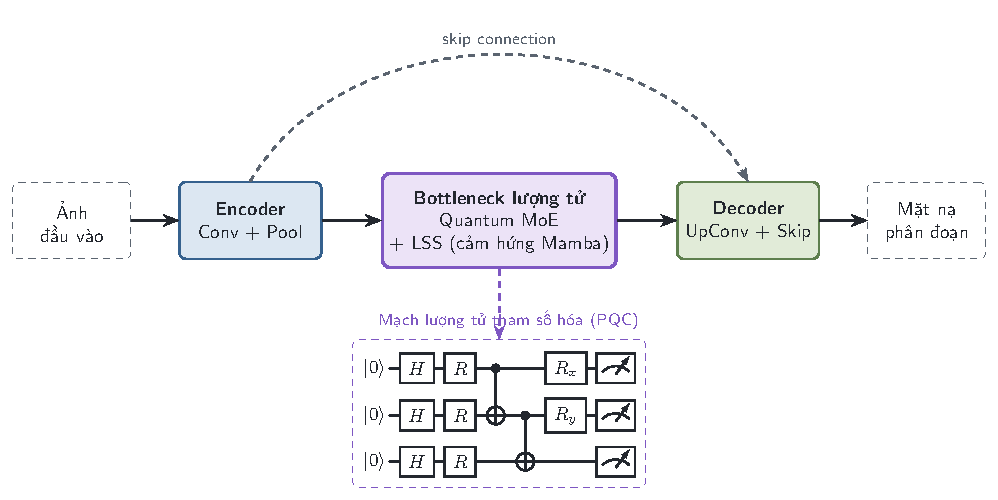
\includegraphics[width=0.92\textwidth]{figures/fig_proposal_overview.pdf}
    \caption{Tổng quan kiến trúc lai lượng tử -- cổ điển đề xuất: bộ khung U-Net với vùng Bottleneck được tăng cường bằng khối hỗn hợp nhánh xử lý lượng tử (Quantum MoE) và khối chuỗi lấy cảm hứng từ Mamba; bên dưới là mạch lượng tử tham số hóa (PQC) minh họa.}
    \label{fig:overview_proposal}
\end{figure}

Quy trình thực hiện dự kiến bao gồm các bước chính sau:

\begin{itemize}

\item Tiền xử lý PH2 và GlaS 2015: resize ảnh và mặt nạ về $192\times256$, chuẩn hóa $[0,1]$, chia mỗi tập theo 5-fold cross-validation.

\item Xây dựng baseline U-Net và các mô hình đối chứng UNet++ \cite{zhou2018unetplusplus}, Attention U-Net \cite{oktay2018attention}, V-Net \cite{milletari2016vnet}, R2U-Net \cite{alom2018r2unet} và mô hình lai dựa trên QuFeX \cite{qufex2025}.

\item Hiện thực các thành phần lượng tử bằng PennyLane (mã hóa biên độ, PQC theo điều kiện NISQ), tích hợp vào cơ chế tự động vi phân của TensorFlow/Keras để huấn luyện đầu-cuối.

\item Xây dựng khối hỗn hợp nhánh xử lý lượng tử đa tỷ lệ (nhánh xử lý có kích thước mảnh và số qubit khác nhau, điều phối bởi mạng định tuyến Softmax và kết nối residual) tiếp nối bởi khối chuỗi lấy cảm hứng từ Mamba tại Bottleneck, cùng khối RDMS ở bộ khung cổ điển, hoàn thiện kiến trúc lai \cite{gu2023mamba}.

\item Huấn luyện (BCE, Adam) và tinh chỉnh siêu tham số; so sánh IoU/Dice với các mô hình đối chứng \cite{du2025qmltutorial}, phân tích hành vi định tuyến và trực quan hóa Seg-Grad-CAM \cite{vinogradova2020seggradcam} để minh họa mô hình tập trung đúng vùng tổn thương.

\end{itemize}

So với phần lớn nghiên cứu trước chỉ ứng dụng mạng lai lượng tử cho phân loại ảnh (đầu ra là một vector nhãn), đề tài hướng đến bài toán phân đoạn ở mức pixel -- phức tạp hơn đáng kể do phải duy trì thông tin không gian chi tiết xuyên suốt kiến trúc -- và khảo sát giá trị của việc kết hợp hỗn hợp nhánh xử lý lượng tử đa tỷ lệ với một khối mô hình hóa chuỗi hiệu quả tại vùng Bottleneck.




    \subsection{Kết quả dự kiến của đề tài}

    \subsubsection{Số liệu định lượng}

    \begin{itemize}
        \item \textbf{Chất lượng phân đoạn:} đánh giá bằng IoU, Dice (DSC), Precision, Recall và Specificity ở mức điểm ảnh, cùng bản đồ phân đoạn trực quan. Kiến trúc lai được kỳ vọng đạt chất lượng cạnh tranh so với các baseline cổ điển (U-Net, UNet++, Attention U-Net, V-Net, R2U-Net) và mô hình lai dựa trên QuFeX.

        \item \textbf{Bản đồ trực quan hóa Seg-Grad-CAM:} minh họa định tính rằng vùng ``chú ý'' của mô hình bám sát vùng tổn thương thực tế.

    \end{itemize}

    \subsubsection{Sản phẩm đầu ra}

    \begin{itemize}
        \item \textbf{Mô hình Hybrid Quantum-Classical U-Net:} nhận ảnh y sinh và sinh bản đồ phân đoạn pixel-level, với khối nhánh xử lý lượng tử và khối LSS tích hợp tại Bottleneck.

        \item \textbf{Tài liệu triển khai:} hướng dẫn cài đặt môi trường (PennyLane, TensorFlow/Keras) và sử dụng mô hình.

        \item \textbf{Mã nguồn chương trình:} mã nguồn tiền xử lý, hiện thực các thành phần, huấn luyện, đánh giá và các script tái hiện kết quả.

    \end{itemize}

    \subsubsection{Các công trình khoa học liên quan}

    \begin{itemize}
        \item \textbf{Báo cáo đề án khóa luận:} Hoàn thiện báo cáo khóa luận với đầy đủ nội dung về cơ sở lý thuyết (kiến trúc U-Net, QML, hỗn hợp nhánh xử lý và mô hình không gian trạng thái), phương pháp thiết kế kiến trúc Hybrid Quantum-Classical U-Net, quy trình thực nghiệm trên hai tập dữ liệu PH2 và GlaS 2015, cùng phân tích và đánh giá kết quả phân đoạn.
    \end{itemize}

    \subsection{Kế hoạch thực hiện}

Kế hoạch thực hiện đề tài được chia theo từng giai đoạn với các mốc thời gian cụ thể như Bảng \ref{tab:plan}.

\begin{table}[H]
\centering
\normalsize
\caption{Kế hoạch thực hiện đề tài}
\label{tab:plan}

\renewcommand{\arraystretch}{1.45}
\setlength{\tabcolsep}{6pt}

\begin{tabular}{|c|p{3.9cm}|p{8cm}|p{3cm}|}
\hline
\textbf{STT} & \textbf{Thời gian} & \textbf{Nội dung công việc} & \textbf{Thành viên} \\
\hline

1 & 01/2026 &
Nghiên cứu U-Net và biến thể; nền tảng Quantum Computing/QML, QuFeX và mô hình chuỗi (Mamba); làm quen PennyLane, TensorFlow/Keras. &
Trực, Vương \\
\hline

2 & 02/2026 &
Khảo sát các mô hình lai quantum--classical; thiết kế sơ bộ khối nhánh xử lý lượng tử đa tỷ lệ và khối LSS tại Bottleneck. &
Trực, Vương \\
\hline

3 & 03/2026 &
Chuẩn bị môi trường; tiền xử lý PH2 và GlaS 2015 (resize $192\times256$, chuẩn hóa $[0,1]$, chia 5-fold). &
Trực, Vương \\
\hline

4 & 04/2026 &
Xây dựng baseline (U-Net, UNet++, Attention U-Net, V-Net, R2U-Net); hiện thực thành phần lượng tử (PennyLane), khối MoE lượng tử, LSS và RDMS, hoàn thiện kiến trúc lai. &
Trực, Vương \\
\hline

5 & 05/2026 &
Huấn luyện và tinh chỉnh siêu tham số; đánh giá IoU/Dice, so sánh với các baseline cổ điển và mô hình lai QuFeX. &
Trực, Vương \\
\hline

6 & 06/2026 &
Phân tích kết quả và hành vi định tuyến; trực quan hóa Seg-Grad-CAM; thí nghiệm bóc tách; hoàn thiện báo cáo. &
Trực, Vương \\
\hline

\end{tabular}

\end{table}


    }

    %TÀI LIỆU TRÍCH DẪN
    \bibliographystyle{IEEEtran}
    \bibliography{sample}
    \nocite{*}

    \vspace{1.5cm}
    \noindent
    \begin{minipage}[t]{0.45\textwidth}
        \centering
        \textbf{XÁC NHẬN CỦA NGƯỜI HƯỚNG DẪN}\\
        \vspace{0.1cm}
        \textit{(Ký và ghi rõ họ tên)}
    \end{minipage}%
    \hfill
    \begin{minipage}[t]{0.5\textwidth}
        \centering
        \textit{TP. Hồ Chí Minh, ngày 11 tháng 03 năm 2026}\\
        \textbf{NHÓM SINH VIÊN THỰC HIỆN}\\
        \vspace{0.1cm}
        \textit{(Ký và ghi rõ họ tên)}
    \end{minipage}

\end{document}